\documentclass[a4paper,english,twoside,10pt]{article}

\usepackage[left=2.5cm,right=2.5cm,bottom=3cm]{geometry}
\usepackage{babel}
\usepackage{amsmath}
\usepackage{makeidx}
\usepackage{array} % Used for `m` table specifier
\usepackage[table]{xcolor} % Used to color the table
% \usepackage{listings}
\usepackage{caption}
\usepackage{csquotes} % Auto open/close quote mark
\MakeOuterQuote{"} % Use quote mark as container for smart quotation system
\usepackage[stretch=10]{microtype} % Better impagination due to micro font shrinking and stretching
\usepackage[justification=centering]{caption}
\usepackage{wrapfig}
\usepackage{tikz}
% \usetikzlibrary{arrows,shapes,calc,babel,positioning,fit}
\usepackage{svg}
\PassOptionsToPackage{hyphens}{url}
\usepackage[breaklinks]{hyperref}
\usepackage[nameinlink]{cleveref}
\usepackage{enumitem}
\usepackage{nameref}
\usepackage{minted}
\usemintedstyle{perldoc}
\usepackage[acronym]{glossaries}
\usepackage{authoraftertitle} % Get title and author available as commands

\newenvironment{scopesetting}{
	\parskip=5pt\par\nopagebreak\centering\sffamily%
	\begin{tabular}{>{\columncolor{cyan!15}}m{2em} >{\columncolor{cyan!15}}m{.8\textwidth}}
	\includesvg{img/scope.svg} & 
} {
	\\
	\end{tabular}
	\par\noindent\ignorespacesafterend%
}

\newenvironment{laptopsetting}{
	\parskip=5pt\par\nopagebreak\centering\sffamily%
	\begin{tabular}{>{\columncolor{red!15}}m{2em} >{\columncolor{red!15}}m{.8\textwidth}}
	\includesvg{img/laptop.svg} & 
} {
	\\
	\end{tabular}
	\par\noindent\ignorespacesafterend%
}
\makeatletter%
\renewenvironment{theindex} {% Inspired by https://tex.stackexchange.com/a/23873/206062
	\@restonecoltrue%
	\section*{\indexname}%
	\@mkboth{\MakeUppercase\indexname}%
			{\MakeUppercase\indexname}%
	\thispagestyle{plain}\parindent\z@%
	\parskip\z@ \@plus .3\p@\relax%
	\columnseprule \z@%
	\columnsep 35\p@%
	\let\item\@idxitem%
	}{}
\makeatother%

\newcommand{\listingautorefname}{Listing}

\hypersetup{
	pdftitle={\MyTitle},
	pdfauthor={\MyAuthor},
	pdfstartview={FitH},
	pdflang={en},
	colorlinks = true,
	linkcolor = blue,
	anchorcolor = blue,
	citecolor = blue,
	filecolor = blue,
	urlcolor = blue
}
\setlist[itemize]{noitemsep}
\setlist[enumerate]{noitemsep}

\makeindex

\graphicspath{{../img/}}

\title{Constructing a dependable side channel data acquisition system for Tektronix 4 Series oscilloscopes}
\author{Federico Cerutti, fce201 \\\href{mailto:federico@ceres-c.it}{federico@ceres-c.it}}

\makeglossaries%
\newglossaryentry{vr} {
    name={VISA Resource},
    description={Any instrument that can be controlled using the \gls{visa} standard}
}
\newglossaryentry{vh} {
	name={VISA Host},
	description={The computer that controls the \gls{vr}}
}
\newacronym{mso}{MSO}{Mixed Signal Oscilloscope}
\newacronym{visa}{VISA}{Virtual instrument software architecture}
\newacronym{ivif}{IVI}{Interchangeable Virtual Instrument Foundation}
\newacronym{scpi}{SCPI}{Standard Commands for Programmable Instruments}
\newacronym{usbtmc}{USB-TMC}{USB Test and Measurement Class}
\newacronym{lxi}{LXI}{LAN eXtensions for Instrumentation}

\begin{document}
\maketitle%
\glsunsetall%

\begin{abstract}
	A successful power analysis attack requires a high-quality and reliable data acquisition system. This report details the construction of a software library to aid in the acquisition of power traces from Tektronix 4 Series \glspl{mso}. The report will also provide information on the different communication protocols used to control test equipment. The reader will be guided through the process of setting up the oscilloscope and acquiring traces.
\end{abstract}

\section{Introduction}
This research project aims to create a reliable setup for collecting side channel data using the Tektronix 4 Series \gls{mso} available at the University of Amsterdam. This oscilloscope has the required high resolution and sampling rate to record power traces, which makes it suitable for side channel analysis projects.

Like most modern test equipment, the oscilloscope supports \gls{visa}, a complex standard that allows to configure laboratory instruments and retrieve data from them. To make this specific oscilloscope easy to use, I created a Python library that uses \gls{scpi} commands, to make the scripting process easier. I faced and solved numerous challenges and instrument-specific bugs during the development, and ultimately achieved a high level of reliability. To demonstrate the effectiveness of this setup, I have prepared example files that showcase its capabilities and robustness.

\glsresetall%
\section{Instrument communication protocols}\label{sec:comm-protocols}
The majority of measurement instruments come equipped with various communication interfaces, with the most common being USB and Ethernet. Multiple protocols exist to facilitate communication with test equipment, and this section will quickly introduce relevant standards and libraries.

\subsection{Transport}
\subsubsection{\texorpdfstring{\gls{usbtmc}}{USB-TMC}}\label{sec:usbtmc}
\begin{wrapfigure}[10]{r}{0.3\textwidth}
	\centering
	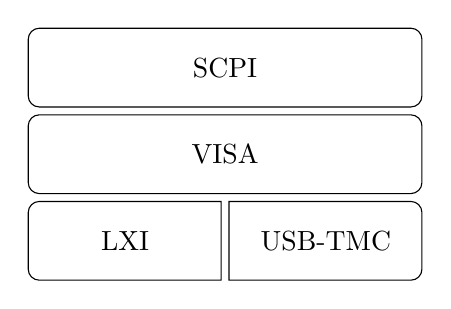
\begin{tikzpicture}
		\draw[rounded corners] (0,2.2) rectangle (5,3.2) node[pos=.5] {SCPI};
		\draw[rounded corners] (0,1.1) rectangle (5,2.1) node[pos=.5] {VISA};
		\draw (2.45,0) -- (2.45, 1) {[rounded corners] -- (0, 1) -- (0,0)} -- cycle;
		\node at (1.23, 0.5) {LXI};
		\draw (2.55,0) -- (2.55, 1) {[rounded corners] -- (5, 1) -- (5,0)} -- cycle;
		\node at (3.78, 0.5) {USB-TMC};
	\end{tikzpicture}
	\caption{Stack of communication protocols}
\end{wrapfigure}
The USB Implementers Forum has defined a standard for USB communication with test equipment. The standard is called \gls{usbtmc} and is supported by most test equipment manufacturers. It defines device descriptors, USB endpoints used for control and data transfer, and encoding of commands and data.

\subsubsection{\texorpdfstring{\gls{lxi}}{LXI}}\label{sec:lxi}
\gls{lxi} is a standard to leverage Ethernet and TCP/IP technologies to control test equipment. The consortium behind \gls{lxi} maintains a set of standards that specify communication protocols (VXI-11, HiSLIP), device discovery features, and REST APIs.

\subsubsection{\texorpdfstring{\gls{visa}}{VISA}}
\gls{visa} is an API that hides the details of the transport layer and provides a common interface to communicate with test equipment. It is a standard developed by the \gls{ivif} and is supported by most test equipment manufacturers. It provides a number of operations (\texttt{read}, \texttt{write}, \texttt{flush}...) and an event system to react to changes.

\subsection{Control}
\subsubsection{\texorpdfstring{\gls{scpi}}{SCPI}}\label{sec:scpi}
\gls{scpi} is a transport-independent API that dictates how to communicate with test equipment. It is a standard developed by the \gls{ivif} and provides a list of commands and queries to control the instrument. It is a text-based protocol, and it is often used on top of \gls{visa} to control test equipment. While it should be a standard, often vendors use different commands and extend it with proprietary features.

\subsection{VISA drivers}
\subsubsection{pyVISA and pyVISA-py}
pyVISA provides python bindings for \gls{visa} libraries: it does not offer any implementation of \gls{visa}, but it relies on third party libraries to provide the functionality. Many vendors provide their own \gls{visa} libraries, some of which are available on linux as well, but are often commercial and not open source. pyVISA-py, in turn, is an open source pure python implementation of VISA that can be used on any platform and interfaces directly with pyVISA. This library lacks some features of the \gls{visa} standard (\texttt{viClear}, \texttt{viClose}...), but it proved to be sufficient for the purpose of this project.

\section{Tektronix 4 Series \texorpdfstring{\glspl{mso}}{MSO}}
The CCI group at the University of Amsterdam has acquired a Tektronix MSO44\footnote{\url{https://www.tek.com/en/datasheet/4-series-mso}} (note: not MSO44B), a 4 Series \gls{mso} with 4 analog channels and a 12-bit ADC at 3.125 GS/s per channel. The ENOB, as stated in the datasheet, is in the range of 8.9 bits (@20MHz) to 7.1 bits (@1.5GHz). These characteristics make it a suitable device for power analysis attacks.

The oscilloscope is equipped with a USB-B 2.0 "device port" (used to control the device from a host computer) and an Ethernet port. There are more USB-A ports, and they can be used for USB HID or storage devices. It supports both \nameref{sec:usbtmc} and \nameref{sec:lxi} communication protocols with \nameref{sec:scpi} commands.

\subsection{Speculations on the firmware}\label{sec:fw-info}
The software architecture of the oscilloscope seems to be more reminiscent of a monolithic, tightly integrated embedded system rather than a modular RTOS. No SDK is provided for this specific device by the vendor, and the only way to control the oscilloscope is through the graphical UI or \gls{visa}.

A quick reverse engineering analysis of the firmware showed that the control of the analog frontend is built into the UI binary, consequently, the \gls{lxi} server also has to go through the UI to execute commands. This becomes problematic when the \gls{lxi} server crashes and stops responding, causing the UI to also become unresponsive, thus requiring manual interaction to reboot the oscilloscope. Crashes will happen in multiple circumstances, but they can mostly be summed up in two categories:
\begin{itemize}
	\item \textbf{Buffer overflows}: The oscilloscope has a limited amount of memory, and it is easy to fill it up when acquiring and transferring multiple traces with the \texttt{CURVE?} command. Speed does not directly affect this issue, as even at speeds as low as 1 trace/s the oscilloscope will eventually crash after \(\sim 300\) traces. I speculate this is due to some internal elaboration buffer that is not being freed. This problem was solved with CurveStream and FastAcq modes (more in \ref{sec:pitfalls}).
	\item \textbf{Network issues}: The TCP stack running on the oscilloscope will stop responding to requests after a variable number of traces in the \(20000\sim 40000\) range, forcing again a manual reboot. This problem was solved by using the USB interface as a backup control interface.
\end{itemize}

\section{Setup}
\subsection{Wiring}
The oscilloscope should be connected to the host computer via both Ethernet and USB. Ethernet is used to control the instrument as well as acquire data, while USB is used as a backup control interface if the Ethernet connection is lost. This is required because, as stated in \ref{sec:fw-info}, the visa implementation on the \gls{vr} is not reliable and often crashes, requiring a reset of the oscilloscope.
\begin{itemize}
	\item \textbf{Ethernet and switch}: The oscilloscope is connected to a router, to which the host computer is also connected. The router provides a DHCP server to assign an IP address to the oscilloscope.
	\begin{scopesetting}
		Utility\ \rightarrow\  I/O\ldots\ \rightarrow\  LAN\newline
		Network Address: Auto\newline
		Apply Changes
	\end{scopesetting}
	\begin{laptopsetting}
		Create a standard network connection with DHCP to the router
	\end{laptopsetting}

	\item \textbf{Ethernet p2p}: The oscilloscope is directly connected to the host computer. The host computer is configured with a static IP address in the same subnet as the oscilloscope. See Tektronix FAQs for more information\footnote{\url{https://www.tek.com/en/support/faqs/im-not-lan-id-establish-peer-peer-connection-my-pc-scopes-ethernet-port-possible}}\\
	\textit{Note}: You need either a crossover cable or a modern network card with Auto MDI-X\footnote{\url{https://en.wikipedia.org/wiki/Medium-dependent\_interface\#Auto\_MDI-X}}.
	\begin{scopesetting}
		Utility\ \rightarrow\  I/O\ldots\ \rightarrow\  LAN\newline
		Network Address: Manual\newline
		Instrument IP Address: 128.181.240.130 (example)\newline
		Subnet Mask: 255.255.255.0\newline
		Apply Changes
	\end{scopesetting}
	\begin{laptopsetting}
		\begin{minted}[breaklines,autogobble]{bash}
			sudo nmcli con add con-name "tek-mso44-p2p" ifname <INTERFACE NAME> type ethernet ip4 128.181.240.131/24
		\end{minted}
	\end{laptopsetting}

	\item \textbf{USB}: Connect the USB-B "device" port on the back of the oscilloscope to the host computer. The oscilloscope will be recognized as a \gls{usbtmc} device.
	\begin{scopesetting}
		Utility\ \rightarrow\  I/O\ldots\ \rightarrow\  USB Device Port\newline
		USB Device Port: ON
	\end{scopesetting}
\end{itemize}

\subsection{Software}
The library is available on PyPI and does not depend on any proprietary software. On Debian 12, the following commands will install the required software:
\begin{minted}[frame=lines,breaklines,autogobble]{bash}
	sudo apt update && sudo apt install python3 python3-pip python3-venv libusb-1.0-0
	python3 -m venv venv
	source venv/bin/activate
	pip3 install pymso4
\end{minted}
Additionally, the USB device needs to be accessible by the user running the script. This can be achieved on Debian adding the user to the \texttt{dialout} group and with udev rules (\texttt{50-newae.rules} is available in the repository at \autoref{app:software}):
\begin{minted}[frame=lines,breaklines,autogobble]{bash}
	sudo -E usermod -a -G dialout $USER
	# Now logout
	cp 50-newae.rules /etc/udev/rules.d/50-newae.rules
	sudo systemctl stop ModemManager && sudo systemctl mask ModemManager
	sudo udevadm control --reload-rules && sudo udevadm trigger
	# Did you logout?
\end{minted}
To test the configuration, run the following python script:
\begin{flushleft}
	\captionsetup{type=listing}
	\begin{minted}[frame=lines,breaklines,autogobble]{bash}
		source venv/bin/activate
		pip3 install psutil # Necessary to discover TCP devices
		pyvisa-shell
		(visa) list
		( 0) USB0::1689::1319::C019654::0::INSTR
		( 1) TCPIP::192.168.1.140::INSTR
	\end{minted}
	\caption{\textit{Note: Your IP might be different}}
\end{flushleft}
There should be at least 2 entries in the output, one for the USB device and one for the Ethernet device.

\section{pyMSO4}
The pyMSO4 library is a python library that provides an interface to control the Tektronix 4 Series \glspl{mso} and acquire power traces. It is built on top of pyVISA and pyVISA-py and provides a high-level interface to control the oscilloscope. It should not be necessary to resort to the programmer manual to configure the basic settings of the oscilloscope.

\subsection{Architecture}
The library has a main class, \texttt{MSO4}, which acts as the main interface to connect to and control the oscilloscope. When a connection to the intrument is initiated, additional classes instances are initialized:
\begin{itemize}
	\item \texttt{MSO4.sc}: The pyVISA resource used to communicate with the instrument
	\item \texttt{MSO4.acq}: Acquisition settings such as horizontal scale and position, sampling rate, waveform length\ldots
	\item \texttt{MSO4.ch\_a}: Per-channel and vertical settings
	\item \texttt{MSO4.trigger}: Trigger settings, different classes implement different trigger types
\end{itemize}

For more details on the available properties and methods, refer to the documentation at \autoref{app:software}.

\subsubsection{Properties}\label{sec:properties}
The configuration is done through properties of the different objects: reading and writing properties will send the appropriate commands to retrieve information or configure settings on the oscilloscope. Some properties (detailed in documentation) are cached locally for performance reasons, which means that they can be read multiple times with no performance penalty, but they might be out of sync with the current oscilloscope settings. This is not a problem when doing long acquisition campaigns, as the oscilloscope is left in a stable state, but it might be a problem during initial setup. For such cases, each class has a \texttt{clear\_cache} method that will force a refresh of all the cached properties on the next access.

\subsubsection{Methods and functions}
The main class has methods to connect to, disconnect from and reset the scope. The library also exposes a function to reboot the oscilloscope via USB, which is useful when the oscilloscope crashes and stops responding to TCP requests. The \texttt{sc} property of the main class is a pyVISA resource, and it can be used to communicate with the oscilloscope directly, be it to send commands not (yet) supported by pyMSO4, or to receive waveform data.

\subsubsection{Acquisition}\index{Acqusition}
The oscilloscope supports different acquisition modes and settings (see \cite[p.~180]{tektronix:mso-help} for more information):
\begin{itemize}
	\item \textbf{Sample}: The default mode, it saves one or more samples during each acquisition interval.
	\item \textbf{Peak Detect}: Saves the highest sample in one acquisition interval and the lowest sample in the next.
	\item \textbf{High Res}\index{Acqusition!High Res}: Maintains the maximum bandwidth possible for the selected sample rate while rejecting aliasing through FIR filters. It guarantees at least 12 bits of vertical resolution, and it sets the maximum real time sample rate to half the maximum sample rate.
	\item \textbf{Envelope}: Displays a waveform record that shows the extremes in variations over several trigger events.
	\item \textbf{Average}: Displays a waveform record that is the average result of several acquisitions to reduce random noise.
	\item \textbf{Roll Mode}: Scrolls sequential waveform points across the display in a right-to-left rolling motion. It starts automatically when the timebase is set to \( \geq 40 \) ms/div.
\end{itemize}

Two additional features related to acquisition are \textbf{FastAcq} and \textbf{CurveStream}. \textbf{FastAcq}\index{Acqusition!FastAcq} (Fast Acquisition) mode is a special mode that minimizes the processing done on the oscilloscope after trace acquisition, thus makes it transfer data to the host computer faster. Skipping the post-processing steps also means the oscilloscope might not behave as expecrted when changing the acquisition settings, see \autoref{item:fastacq} for more information.
\textbf{CurveStream}\index{Acqusition!CurveStream} is a special mode that allows the oscilloscope to send the acquired waveform data directly to the host computer with minimal buffering. This is useful when the oscilloscope is used to acquire numerous waveforms in a short time, as it minimizes the risk of the oscilloscope crashing due to buffer overflows. See \autoref{item:curvestream}.
The combination of FastAcq and CurveStream modes is the most efficient way to reliably acquire an indefinite number of traces from the oscilloscope.

\subsubsection{Triggers}
The trigger type is selectable through the \texttt{trigger} property of the main \texttt{MSO4} class. The oscilloscope supports multiple advanced triggering options, including some protocol-specific triggers, see \cite[p.~159]{tektronix:mso-progman}\cite[p.~121]{tektronix:mso-help} for more information. The following trigger types are currently available:
\begin{itemize}
	\item \textbf{\texttt{MSO4EdgeTrigger}}: Edge trigger will trigger on a rising, falling, or both edges of a signal.
	\item \textbf{\texttt{MSO4WidthTrigger}}: Pulse width trigger, will trigger when a signal pulse width is less than, greater than, equal to, or not equal to a specified pulse width.
\end{itemize}

Additional triggers can easily be implemented extending the \texttt{MSO4TriggerBase} base class, which already supports the common trigger settings.

\subsection{Examples}
The library comes with a few examples to demonstrate its usage in the \texttt{examples} directory
\begin{itemize}
	\item \texttt{ex0\_square\_capture.ipynb} demonstrates how to capture a trace of the calibration square wave from the oscilloscope (see \autoref{fig:square-wave-setup}).
	\item \texttt{ex1\_cw305\_capture.ipynb} demonstrates how to capture a trace of the power consumption of the CW305 target board\cite{cw305:spec} when triggering on analog channel 2 (see \autoref{fig:cw305-setup}).
	\item \texttt{ex2\_cw305\_endurance.py} demonstrates how to run a long acquisition campaign and handle disconnections and crashes with the CW305 target board\cite{cw305:spec}.
\end{itemize}

Further information on the hardware setup to run these examples can be found in the examples source files as well as in the documentation at \autoref{app:software}.

\begin{figure}[htbp]
	\centering
	\begin{minipage}{.5\textwidth}
	  \centering
	  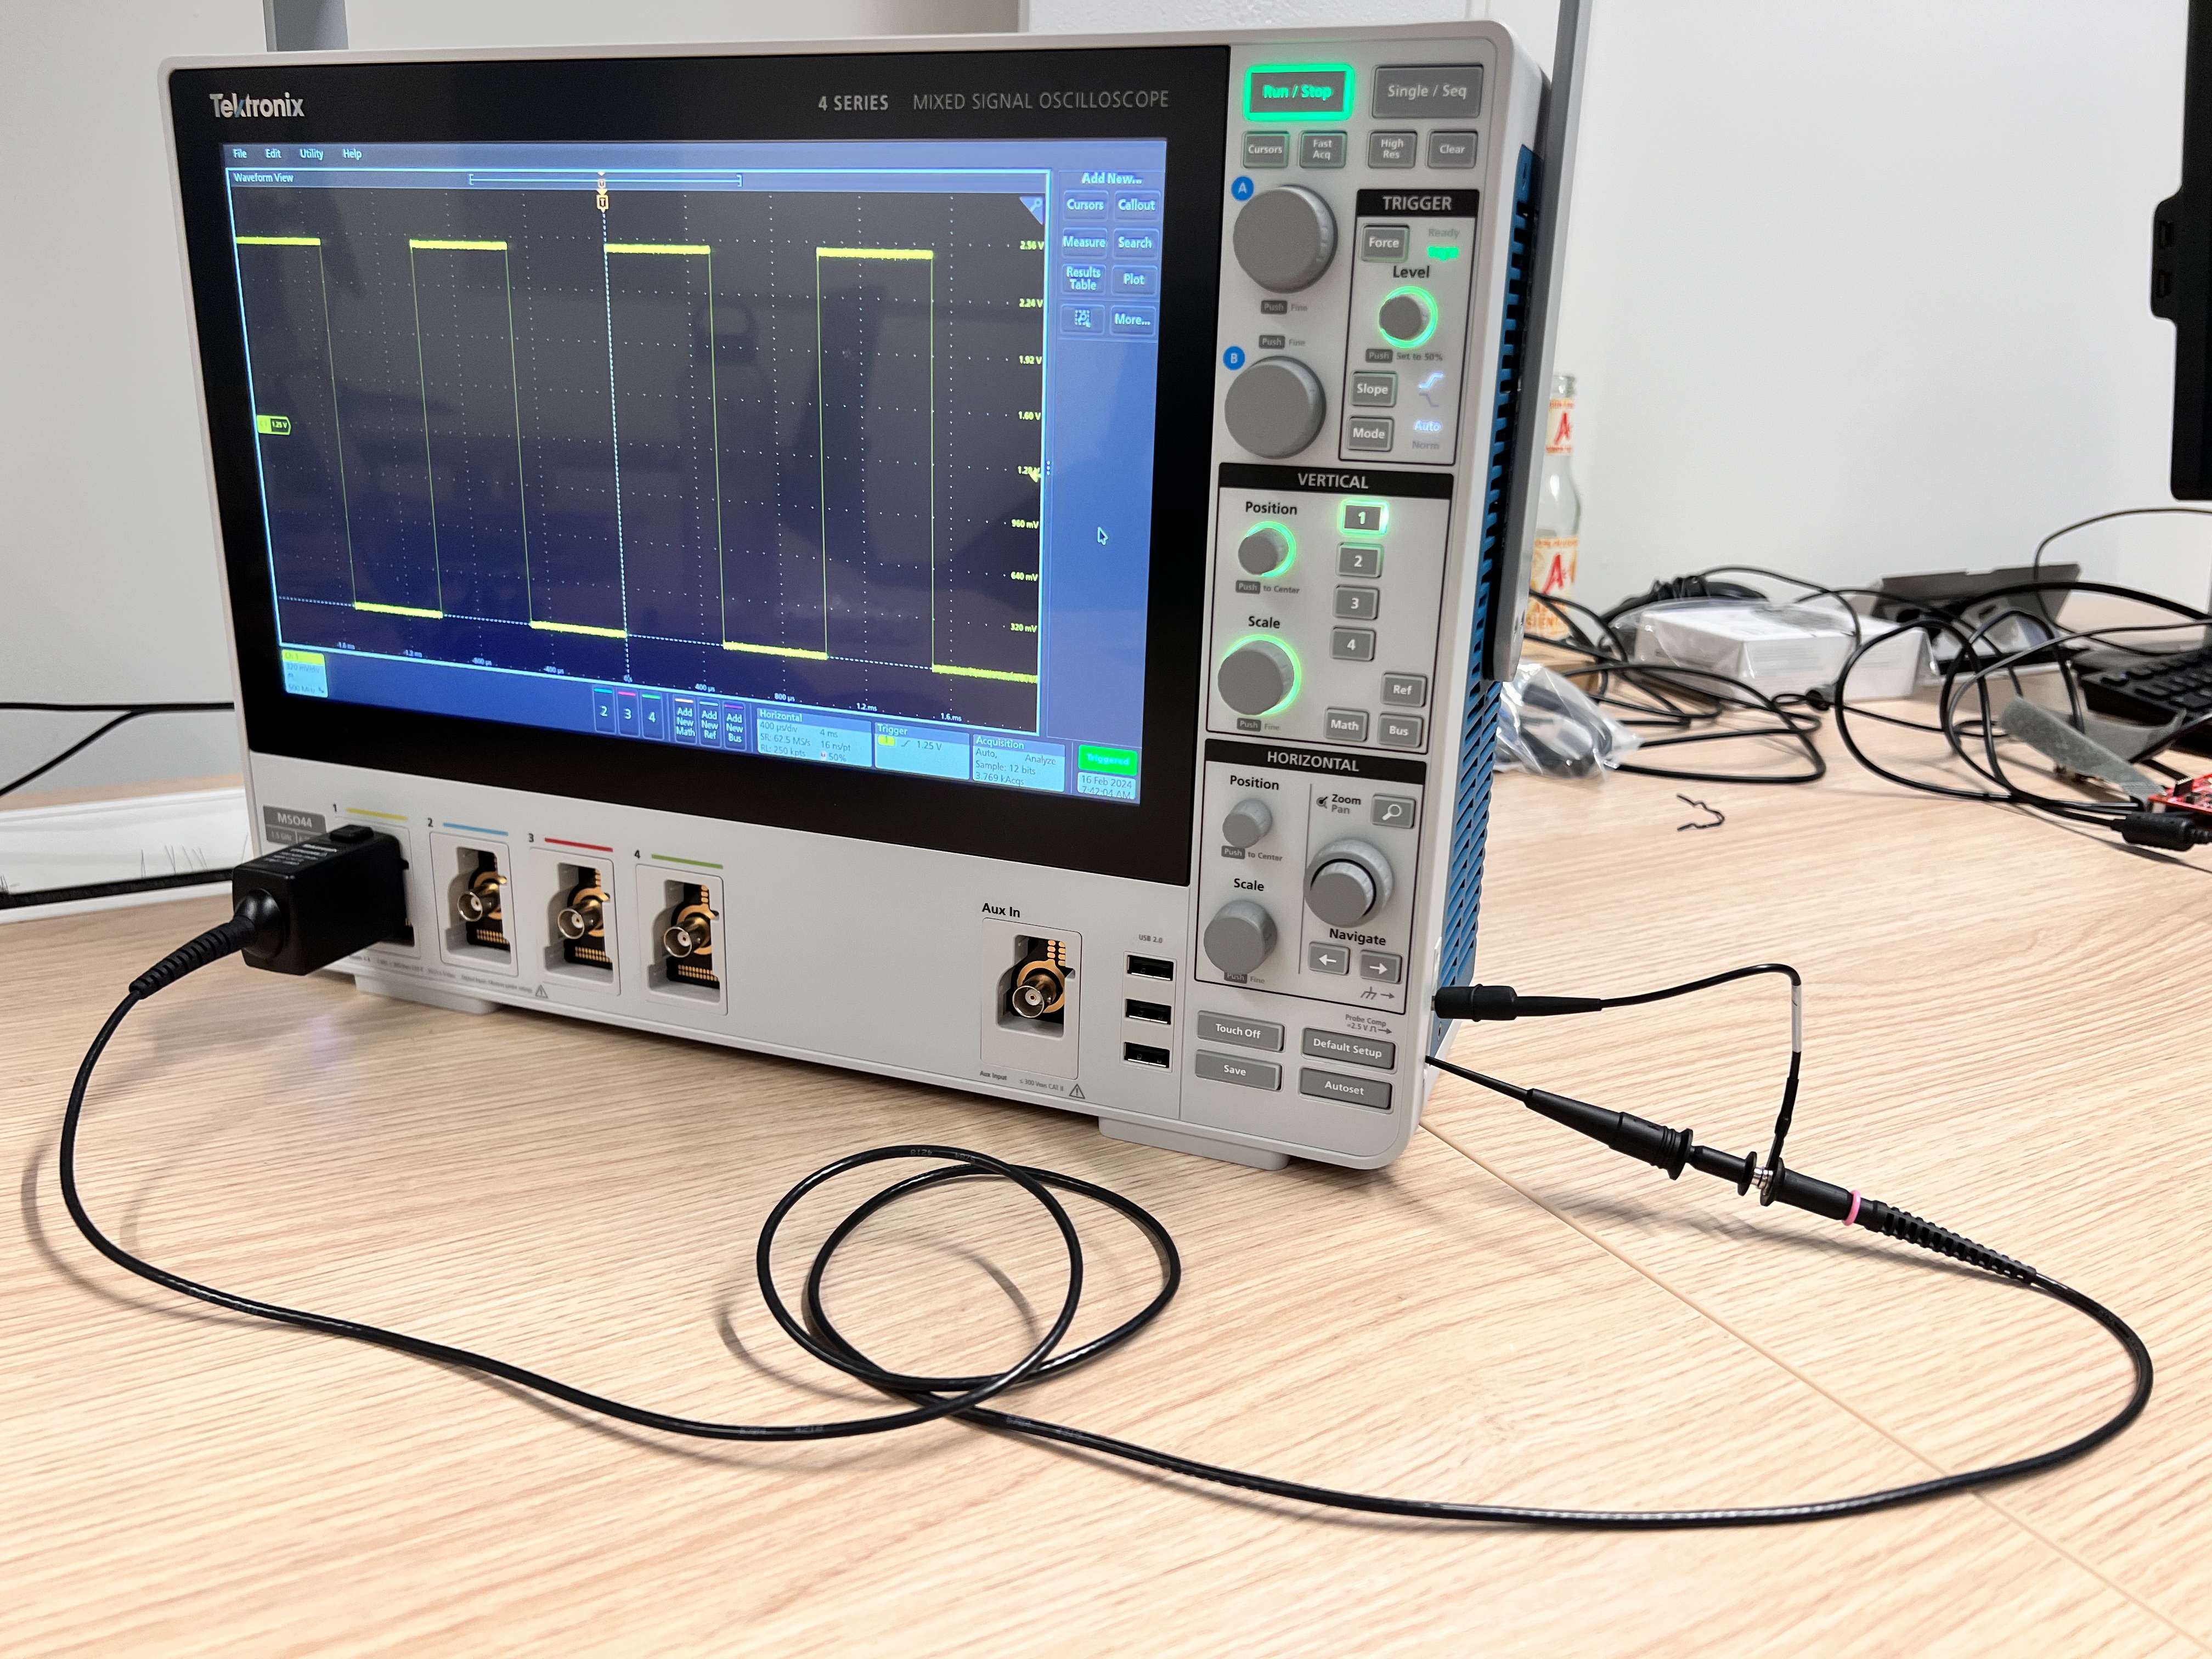
\includegraphics[trim=50 0 50 0,clip,width=.9\linewidth]{../docs/_static/square_wave_setup.jpg}
	  \captionof{figure}{Square wave setup}
	  \label{fig:square-wave-setup}
	\end{minipage}%
	\begin{minipage}{.5\textwidth}
	  \centering
	  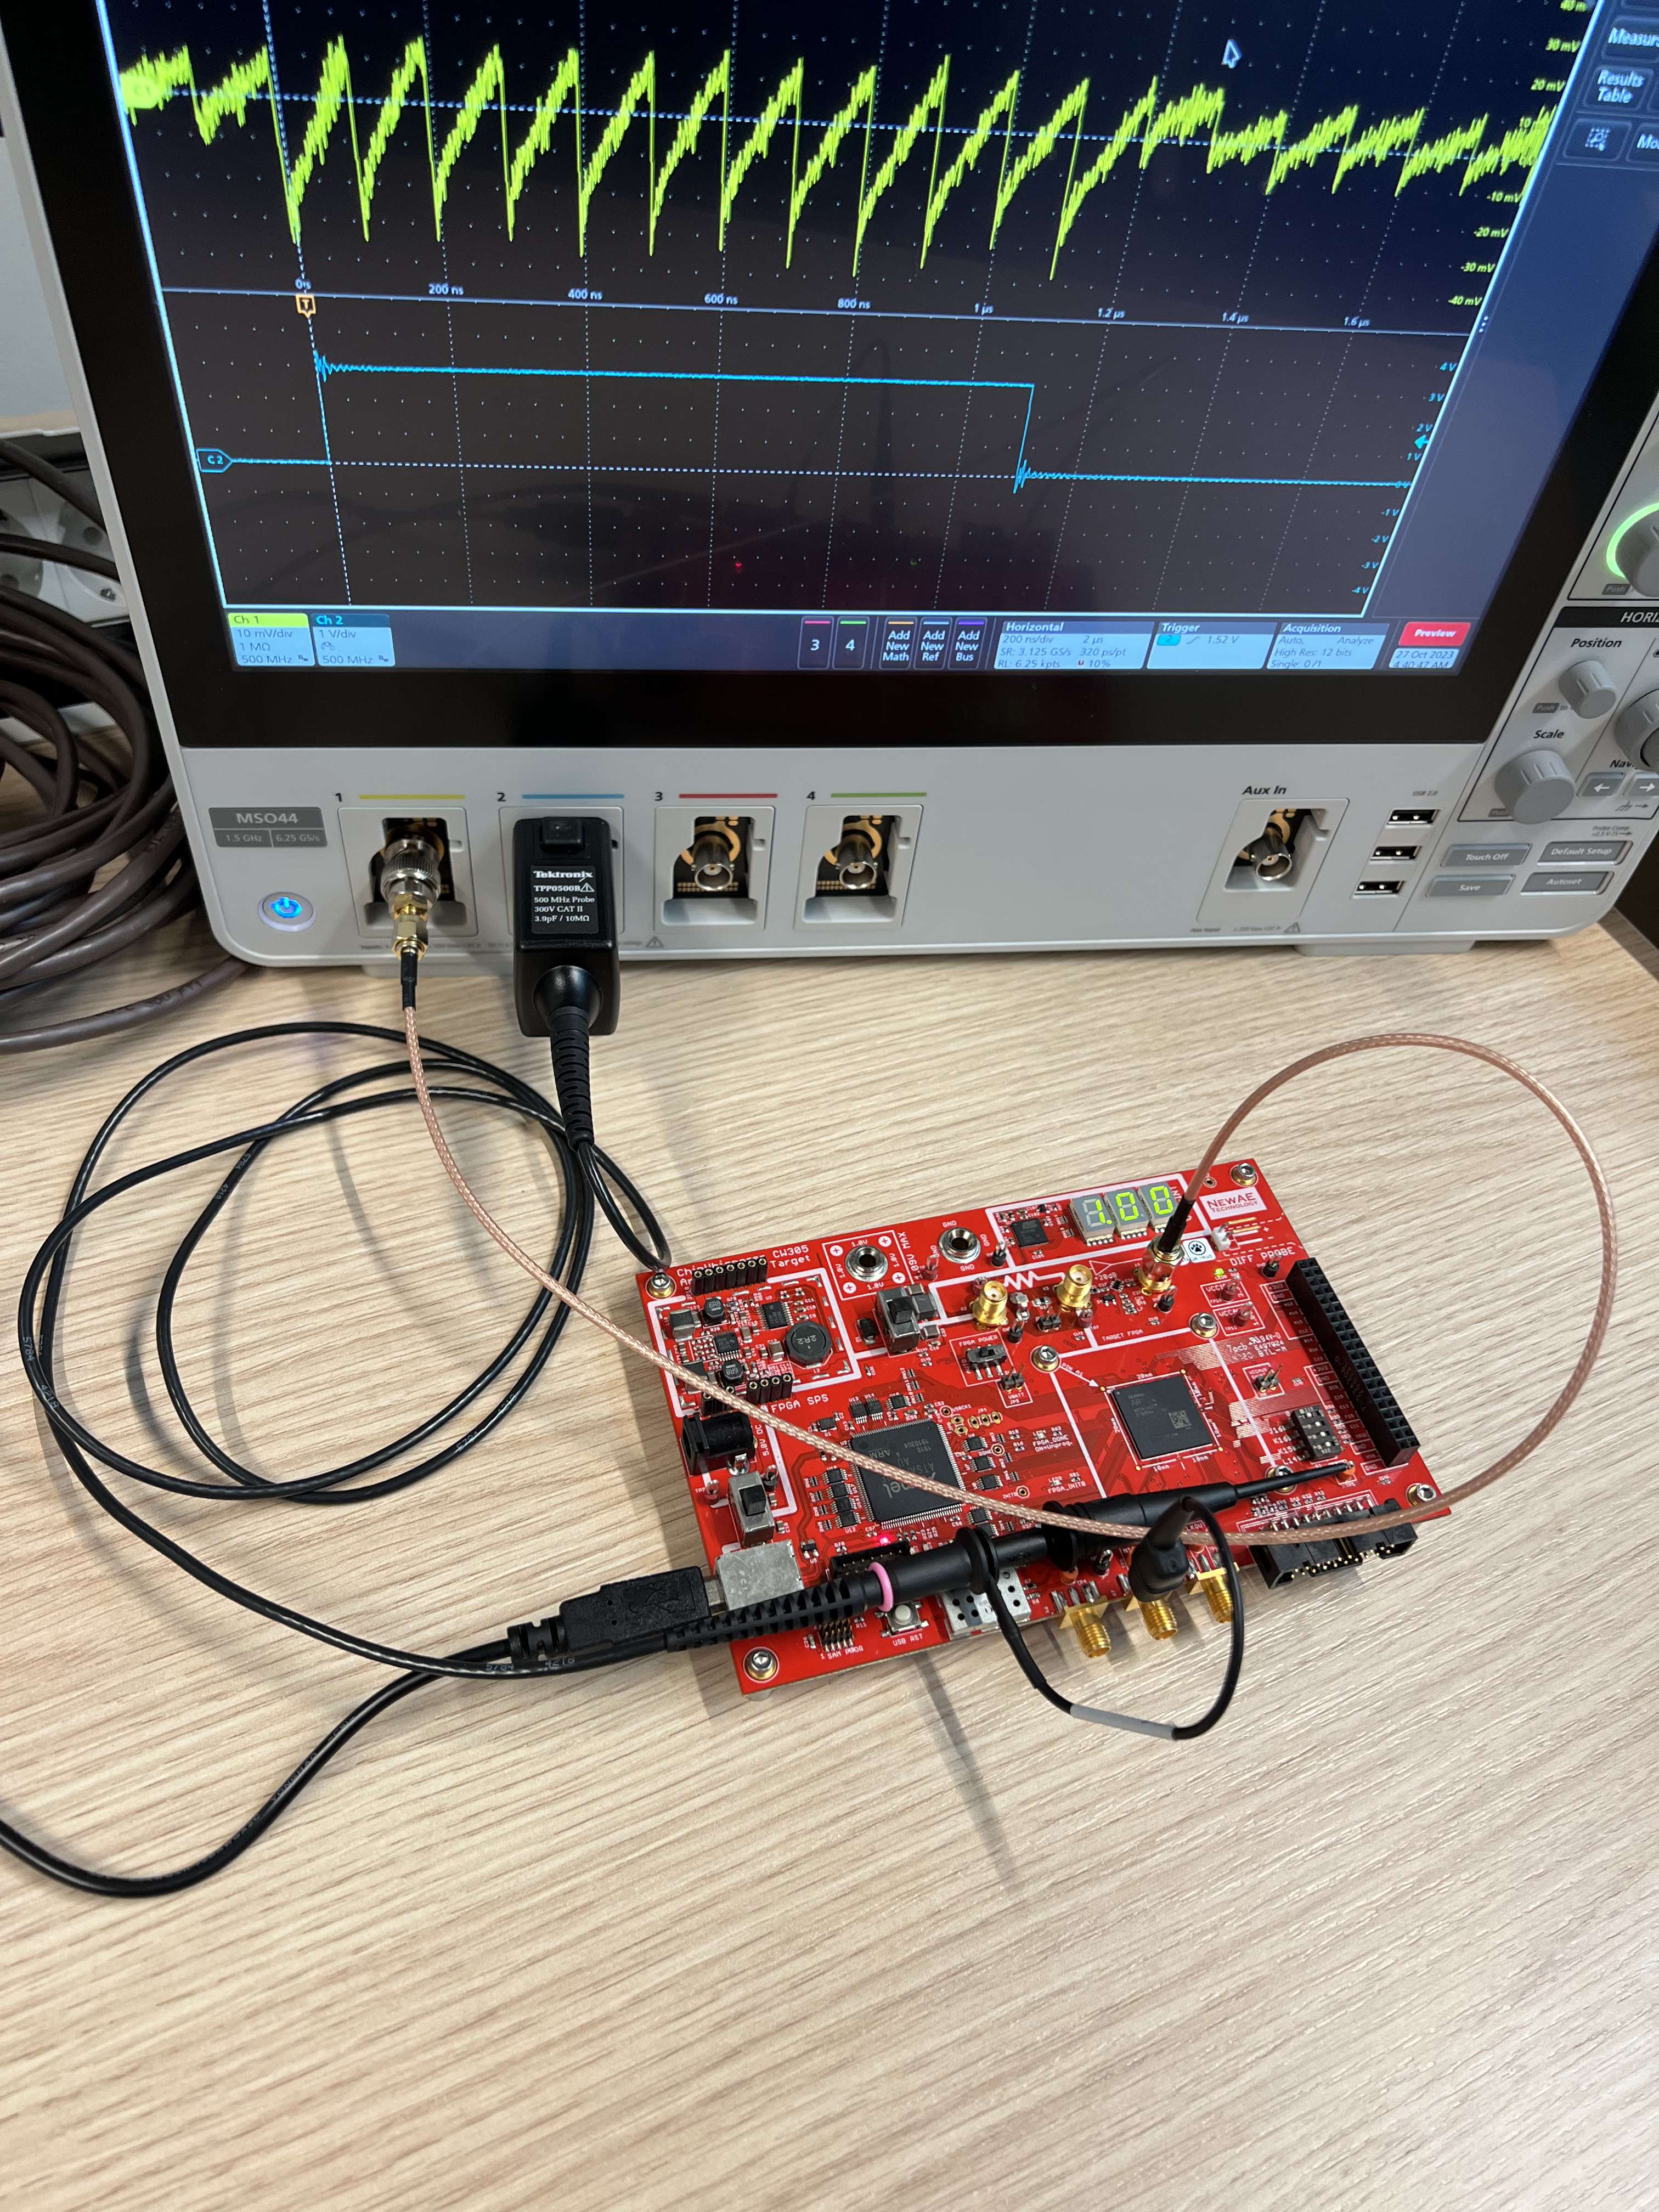
\includegraphics[trim=0 700 0 0,clip,width=.9\linewidth]{../docs/_static/cw305_setup.jpg}
	  \captionof{figure}{CW305 setup}
	  \label{fig:cw305-setup}
	\end{minipage}
\end{figure}

\subsubsection{Minimal example}
After connecting the probe on channel 1 to the calibration square wave output, and pressing the Autoset button, the following code will capture a trace of the signal as seen on the oscilloscope screen:
\begin{flushleft}
	\captionsetup{type=listing}
	\begin{minted}[frame=lines,breaklines,autogobble]{python3}
		import pyMSO4
		mso44 = pyMSO4.MSO4(trig_type=pyMSO4.MSO4EdgeTrigger)
		mso44.con(ip="128.181.240.130") # Using p2p ethernet connection
		mso44.ch_a_enable([True, False, False, False]) # Enable channel 1
		mso44.acq.wfm_src = ['ch1'] # Set waveform source to channel 1
		mso44.acq.wfm_start = 0
		mso44.acq.wfm_stop = mso44.acq.horiz_record_length # Get all data points
		wfm = mso44.sc.query_binary_values('CURVE?', datatype=mso44.acq.get_datatype(), is_big_endian=mso44.acq.is_big_endian)
	\end{minted}
	\caption{pyMSO4 minimal example}
\end{flushleft}

\subsection{Performance}
With the code in \texttt{ex2\_cw305\_endurance.py}, the oscilloscope was able to acquire \(1\,119\,856\) waveforms over a period of \(120\,119\) s (\(\sim33\) hours), which corresponds to a frequency of \(9,3\) Hz. The oscilloscope was connected to the host computer via Ethernet and USB, and the acquisition was done with FastAcq and CurveStream modes enabled.

\subsection{Pitfalls}\label{sec:pitfalls}
\gls{visa} is a complex standard with asynchronous operations, events, and multiple layers of abstraction. The \gls{visa} standard is not always implemented correctly by vendors, and the pyVISA-py library is not a complete implementation of the standard. This means there are multiple gray areas and "should's" in the documentation that are not always true. For example, some commands simply do not work as stated in the programming manual\cite{tektronix:mso-progman}. Here are some of the issues encountered during the development of the library:
\begin{enumerate}[label=\textbf{P.\arabic*},ref=P.\arabic*]
	\item \textbf{Property caching}: As mentioned in \ref{sec:properties}, some properties are cached locally for performance reasons. This can lead to unexpected behavior when the oscilloscope is being controlled both by the library and the UI.\\
	\textit{Solution:} Use the \texttt{clear\_cache} method to force a refresh of all the cached properties on the next access.
	\item \textbf{Synchronization issues 1}: It is often the case that swapping the order of two instructions in the code will result in a different behavior of the oscilloscope. This is due to the fact that the oscilloscope is not always able to keep up with the commands sent to it, regardless of what stated in the manual\cite[p.~1915]{tektronix:mso-progman}, and some commands might not execute in time.\\
	\textit{Solution:} Explicit delays might help.
	\item \textbf{Synchronization issues 2}: Some long-running commands can set the bit 0 of the \texttt{SESR} register when the execution is complete through the \texttt{*OPC} command (also see \autoref{item:opc}).\\
	\textit{Solution:} A list of commands that support this signaling system is available in the manual\cite[t.~3-3]{tektronix:mso-progman}.
	\item \textbf{\texttt{*OPC}}\label{item:opc}: The non-query version of \texttt{*OPC} does not work as stated in the manual\cite[p.~1001]{tektronix:mso-progman}: complete bit is not set in the register. The query version \texttt{*OPC?} works as expected.
	\item \textbf{Buffer overflows}\label{item:curvestream}: As stated in \ref{sec:fw-info}, extensive usage of the \texttt{CURVE?} command will eventually crash the oscilloscope.\\
	\textit{Solution:} Use CurveStream mode, which sends data directly to the host with minimal buffering
	\item \textbf{CurveStream}: Using CurveStream mode without FastAcq mode will result in the oscilloscope crashing just like with the \texttt{CURVE?} command.\\
	\textit{Solution:} Enable FastAcq mode.
	\item \textbf{FastAcq}\label{item:fastacq}: The length of the waveform retrieved from the oscilloscope can be freely configured, but its actual value will not be updated on the oscilloscope's end until a normal acquisition is performed. This is (probably) due to the optimizations done in FastAcq mode that skip many of the post-procesing steps that would normally happen in a normal acquisition.\\
	\textit{Solution:} Force a trigger after setting the length of the waveform and check if the data length has been updated.
	\item \textbf{Oscilloscope not responding via TCP}: The oscilloscope might constantly timeout or kill the TCP session after a variable number of traces even when all above issues are addressed. It will also reject any further attempt to initiate a new connection.\\
	\textit{Solution:} Use the USB interface to reboot the device with \texttt{pyMSO4.pyMSO4.usb\_reboot}.
\end{enumerate}

The list above is in no way exhaustive, it is just a collection of issues encountered during the development of the library that I can remember at the time of writing.

\clearpage%
\printglossary[type=\acronymtype,nogroupskip]%
\printglossary[nogroupskip]%
\printindex%
{
\raggedright%
\nocite{ico:oscilloscope}
\nocite{ico:laptop}
\bibliographystyle{IEEEtran}
\bibliography{bibliography}
}

\clearpage%
\appendix%
\section{Software}\label{app:software}
Source code of pyMSO4 python library can be found at \url{https://github.com/ceres-c/pyMSO4}.

\noindent Auto generated code documentation is available at \url{https://ceres-c.it/pyMSO4/}.
\section{Hardware}\label{app:hardware}
\subsection{Bill of materials}
The setup was tested with the following components:
\begin{itemize}
	\item \(1 \ \times\) MSO44 oscilloscope (Firmware version \textit{non-windows V2.0.3.950})
	\item \(1 \ \times\) Debian 12 computer with 1 USB-A port and 1 Ethernet port
	\item \(1 \ \times\) Xiaomi Mi Router 4A with OpenWRT (not necessary if using ethernet p2p)
	\item \(2 \ \times\) Ethernet cables (1 if using ethernet p2p)
	\item \(1 \ \times\) USB-A to USB-B cable
\end{itemize}
Additionally, to communicate with the CW305\cite{cw305:spec} target board, the following components are required:
\begin{itemize}
	\item \(1 \ \times\) SMA-SMA cable
	\item \(1 \ \times\) SMA-BNC adapter
	\item \(1 \ \times\) BNC probe
\end{itemize}
\section{If your \texttt{uid} is not 0, you don't own it}
Being frustrated by the aforementioned memory issues with the \texttt{CURVE?} command, I started analyzing a firmware update package with a friend of mine\footnote{\url{https://github.com/CarloMara}}. We quickly assessed it was a linux squashfs filesystem, and we were able to extract the content of the archive to check for any low hanging fruits. We found that network configuration settings configured through the Web UI were passed as parameters to a shell file from the CGI backend. These parameters were not sanitized (\autoref{fig:exploit-sh}), and we were able to obtain arbitrary code execution as root injecting commands through an HTTP proxy (\autoref{fig:exploit-burpsuite}).

\begin{figure}[htbp]
	\centering
	\includegraphics[width=\textwidth]{img/exploit\_sh.png}
	\caption{Exploit entry point in \texttt{scopeapp\_install/scopeapp\_tar/LXI\_RefDesign/Scripts/LinuxIfConfig.sh}}\label{fig:exploit-sh}
\end{figure}

\begin{figure}[htbp]
	\centering
	\includegraphics[width=\textwidth]{img/exploit\_burpsuite.png}
	\caption{Injecting commands from the proxy}\label{fig:exploit-burpsuite}
\end{figure}

Code execution was not sufficient to obtain a shell on its own because the most common linux utilities available in the firmware did not allow for easy shell access. Nevertheless, we noticed the presence of a python 2.7 interpreter, and that we could run a script from USB storage. We then wrote a simple script that would start a socket server and echo the output of any command sent to it.

\begin{figure}[htbp]
	\centering
	\includegraphics[width=\textwidth]{img/exploit\_id.jpg}
	\caption{got root}\label{fig:exploit-id}
\end{figure}

Additionally, we noticed that external storage is mounted with read/write/execute permissions, thus it would be trivial to compile a statically linked sshd binary and run it from the oscilloscope. We did not pursue this any further as I managed to work around the memory issues with CurveStream mode, but it would be interesting to continue this analysis and, potentially, build a small SDK to run acquisition campaigns directly on the oscilloscope.
\end{document}
